\documentclass[12pt]{report}
\usepackage{amsmath}
\usepackage{graphicx}
\usepackage{palatino}

\graphicspath{{./}{figs/}}

\def\v#1{\vec{#1}}
\def\h#1{\widehat{#1}}
\def\o#1{\bar{#1}}
\def\C#1{{\cal{#1}}}

\newcommand{\eqn}[1]{equation (\ref{#1})} 
\newcommand{\eqnn}[1]{(\ref{#1})}
\newcommand{\fig}[1]{Figure \ref{#1}}
\newcommand{\BF}{BlobFlow}

\newcommand{\OneFigure}[1]{\begin{center}
\
\ \epsfysize=2.5in \epsfbox{#1}\ 
\end{center}}

\title{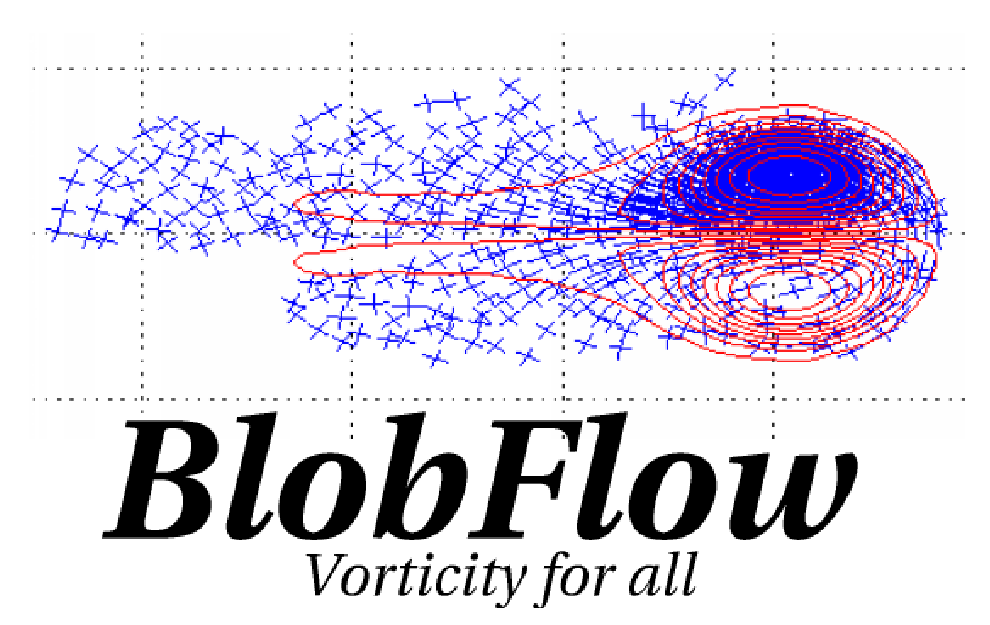
\includegraphics{figs/BlobFlow_logo} \\
 A high order vortex method for viscous flows \\
User's Guide \\ Version $1.0$ for BlobFlow v3.x.}
\author{Louis F. Rossi}
\date{September 2009}

\oddsidemargin0in
\textwidth6.5in

\begin{document}

\maketitle

\chapter{Formalities}

\section{Copyright}

Copyright \copyright \ 2001, 2009 Louis F. Rossi. 

Permission is granted to copy, distribute
and/or modify this document under the terms of the GNU Free Documentation
License, Version 1.1 or any later version published by the Free Software
Foundation; with the Invariant Sections being 
\begin{itemize}
\item Formalities;

\item Preliminaries;

\item Building \BF;

\item Using \BF.

\end{itemize}
A
copy of the license is included in the appendix entitled "GNU Free
Documentation License".

\section{History}


\begin{tabular}{lll}
August & 2000 & Original draft written by L. F. Rossi for 
\BF~v1.0. \\
July & 2001 & Original draft written by L. F. Rossi for 
\BF~v2.01. \\
August & 2001 & Revised draft written by L. F. Rossi for 
\BF~v2.01. \\
August & 2009 & Revised draft written by L. F. Rossi for 
\BF~v3.x. \\
\end{tabular}

\section{Changes since v2.x}

Many algorithmic details have changed in \BF~since the v2.x release in
2001.  Some of these changes do not affect how one sets up the runs the program,
but two elements will have a major impact on users:
\begin{itemize}
\item Accelerated Biot-Savart evaluation.  The earlier version of \BF~used an
asymptotic Biot-Savart evaluation for elliptical Gaussian basis functions.  The
current version uses a new spectral interpolation algorithm that offers
improvements in speed and accuracy at a cost of requiring look-up tables
\cite{platte-rossi-mitchell}.

 \item Single-step integration.  Earlier versions of BlobFlow used high order
Adams family integrators.  The current version uses a single step Runge Kutta
method.  My reason for making the change is that it simplified all other
portions of the algorithm to use a single step method so that one would not need
to treat trajectories of blobs when removing or adding them to a simulation. 
This change makes it much easier to add and remove features from the code.

\item Splitting and merging has been completely replaced by field interpolation.
 Field interpolation is a global means of replacing one configuration of
particles with another while inducing controllably small errors.  While
localized splitting and merging was an elegant approach, I have found that using
a  reverse heat equation solver is far more effective and accurate
\cite{barba-rossi}.
\end{itemize}


\chapter{Preliminaries}

\section{This software is free.}

\BF~is a computer algorithm known as an elliptical corrected core
spreading vortex method (ECCSVM).  This software is free is many senses.
\begin{itemize}
 \item  This software is commercially free.  Anyone may download and use this
code at no cost.
\item This software is conceptually free.  There is a transparent path between
input and output.  Anyone may examine the source code to gain a better
understanding of how it functions.
\item This software is intellectually free.  I want others to use my code.  I
place no obligations on the user of the code beyond the open source license
itself.
\end{itemize}

The name ``BlobFlow'' was trademarked to
represent my particular distribution, but the trademark is no longer maintained.
 
The code distributed under the name \BF~is open source.
Anyone is free to copy, modify and use it, as long as they abide by the
terms of the attached copyright.  If you would like to share modifications and
patched with me, I will happily include them in my source code.

\section{What is a vortex method?  Will it solve my problem?}

A vortex method is a numerical algorithm for calculating fluid flows.
\BF~is restricted to two-dimensional, incompressible, viscous flows
though I hope to develop a three dimensional version one day.
Vortex methods are effective for flows dominated by isolated regions of
vorticity.  Examples include vorticity shedding from bluff bodies,
simulation of coherent vortical structures, boundary layers, jets and so
forth.  There are situations where vortex methods would not be a good
choice, so it is best to analyze the problem for choosing this algorithm.

\BF~is based on the elliptical core spreading vortex method.  A vortex
method is an algorithm that approximates the vorticity field, $\omega$, 
of a fluid flow
as a linear combination of moving, localized basis functions, sometimes
called {\em blobs}.
\begin{eqnarray}
&& \omega(\v x,t) = \sum_{i=1}^N g(\v x;\gamma_i,\v x_i,\sigma_i,a_i,\theta_i)
\nonumber \\
&& g(\v x;\gamma_i,\v x_i,\sigma_i,a_i,\theta_i) = \hfill \nonumber \\
&& {\gamma_i \over 4 \pi \sigma_i^2}
\exp\left\{
-{[c_i (x-x_i)+s_i (y-y_i)]^2/a_i^2 +
[-s_i (x-x_i)+c_i (y-y_i)]^2 a_i^2
\over
4 \sigma_i^2}
\right\}
\label{basis-fn}
\end{eqnarray}
where the parameters $\v x_i$, $\sigma_i$, $a_i$ and $\theta_i$ are
functions of time.  The evolution equations for these quantities which can
be found in \cite{rossi-deform-1,rossi-deform-2}, are related to the flow
velocity and the
derivatives of the flow velocity.  The centroid of the blob is $\v
x_i$. The width, aspect ratio and orientation of the blob is $\sigma_i$.
$a_i^2$ and $\theta_i$, respectively.  The total number of blobs, $N$, is
often referred to as the {\em problem size} and can be compared to the
number of mesh points in a finite difference computation.

Where finite
difference schemes use mesh points as the fundamental computational element,
a vortex method uses moving basis functions so that there is no grid imposed
upon the problem.  Schemes using elements that move with the flow are called
Lagrangian schemes because they are formulated in Lagrangian coordinates
that move with the fluid rather than Eulerian coordinates which are fixed in
some laboratory reference frame.  This is both a strength and a weakness.
One of the main strengths is that the method is naturally adaptive.
Vorticity moves through the domain as dictated by the governing
Navier-Stokes equations.  The main disadvantage is the lack of a regular
grid.  A regular grid has more than aesthetic advantages.  Having a regular
grid means that memory can be allocated in a geometrically relevant way.
In a Lagrangian scheme, no such assumptions can be made.

\chapter{Building \BF}

\section{Requirements}

I tried to make \BF~as simple as possible to use.  This is short list of what
you will need.

\begin{itemize}
\item The source code.
\item The lookup table binary files for \BF.
 \item A C compiler.
\item The \texttt{lapack} and \texttt{blas} libraries.  These libraries freely
available and easy to install.
\item The GNU make utility or a compatible make utility.  The make utility is
ubiquitous.
\item If you choose to use multiple cores with the MPI option, you will need
the MPI libraries.  Again, these are freely available to download.
\end{itemize}


\section{For the impatient}

\BF~is built using the GNU make utility.  One can simply unpack the distribution
and build it.

\begin{verbatim}
tar xzf blobflow.tgz
cd BlobFlow_3.x
make eflow
\end{verbatim}

You will also need to unpack the look-up tables somewhere.  When you run \BF,
you will need to tell \BF~ where to find the look-up tables.

\begin{verbatim}
# Remember you put these files.
tar xzf domain.tgz
\end{verbatim}

\section{Build options}

\BF~is written entirely in ANSI C.  While it was developed on Unix and Linux
platforms, there are no machine -pecific functions in the code.  The code is
distributed with a vanilla Makefile for the Unix {\em make} utility.

\BF~uses conditional compilation so that users can customize the
executable for special situations.  The most common one can be compiled into the
code through the make command, but some require editing the CFLAGS arguments in
the makefile.
\begin{enumerate}

\item Use the Message Passing Interface (MPI) to parallelize across multiple
processors (mpi=on): Many aspects of the algorithm are parallelizable, and
this feature spreads the work among many processors.  To use this
capability, you must install and configure a version of MPI (available at {\tt
http://www.openmpi.org} for instance) properly on the machines that you wish to
use.
You should also familiarize yourself running programs with MPI calls.  It's
easy to learn and worth the time.  \BF~uses two algorithms under MPI.
If only two processors are available, it uses a peer based scheme to evenly
spread the work between the two processors.  If there are more than two
CPU's available, \BF~uses a worker-manager algorithm with a receive and
dispatch scheme to balance the work amongst all available processors.  This
means that one process oversees activities
without doing any number crunching.  In principle, a two processor peer-based
system will run about as fast, and perhaps a little faster, than a three
processor manager-worker system.  However, if one has $N+1$ processors, the
total computation time should scale like $1/N$ for small groups of processors.

\item Cache resorting (CFLAGS = -DCACHERESORT): Though CPU speeds have increased
substantially in recent years, front side bus and memory speeds have not
kept pace.  In fact, most of the memory is orders of
magnitude slower than the CPU.  A small reserve, called cache, is fast
memory.  When instructions and data for calculations are resident in this
cache, codes will run substantially faster.  Computer architects and
compiler authors are pretty crafty and optimizing the use of cache, but
there are also ways to write code to take advantage of cache.  I have
attempted to do this in \BF~but have found that cache awareness has
little or no impact on the platforms I have used.  However, since cache
structure is machine dependent, I have left the feature in place.

\item Direct summation (CFLAGS = -DNOFASTMP):  To accelerate computations, the
program uses a modified fast multipole summation for the velocity and velocity
derivative calculations.  While this is accepted practice, it can induce
small but quantifiable errors.  This can be disabled with the NOFASTMP flag.

\end{enumerate}

To use these options either together or separately, under the GNU make
utility, you just set the switches on the command line. For instance,
\begin{verbatim}
make mpi=on xantisymm=on
\end{verbatim}
will build an executable with both options.

If you do not have the GNU make utility on your system, you must edit the
vanilla Makefile.  It is easy to do.  Just follow the instructions and
comment/uncomment the appropriate sections of flags.

\chapter{Using \BF}

\section{For the impatient.}

A fluid simulation is not something for the impatient.  There are some
sample files included with the distribution.  These should all work if you
set your environment variables to point at the correct simulation files.

Even with reasonable initial conditions and physical
parameters,
\BF~might crash.  If the computational parameters
are two coarse to capture the relevant physical effects, the computational
representation may overflow, divide by zero or use up all the memory.
Strong numerical tools are fast and accurate but they are not necessarily 
bulletproof.

\section{Command line options}

\BF~is run from the command line with three mandatory parameters.
\begin{verbatim}
eflow -inputdir <INPUT_DIR> -config <CONFIG_FILE> -domdir <DOM_DIR>
\end{verbatim}
\BF~will look in the directory INPUT\_DIR for the simulation and control files,
with names CONFIG\_FILE.sim and CONFIG\_FILE.ctl, respectively.  \BF~also uses a
lookup table when it evaluates the velocity field contributions from the
deformed blobs \cite{platte-rossi-mitchell}.  It expects to find these files in
the directory DOM\_DIR.  (This is where you unpacked the \texttt{domain.tgz}
archive.)

\section{The simulation and control files}

There are two groups of parameters for \BF.  The first group is the
physical description of the problem such as the fluid viscosity and the
initial conditions.  The information in this file only describes the fluid
experiment, and has nothing to do with \BF, which is one means of
approximating the outcome of the experiment.  BlobFlow performs some
elementary tests to make sure that the essential parameters are set
properly before the simulation begins, but this is by no means
bulletproof, and it is not recommended that this feature be used to
assure that control or simulation parameters are self-consistent.
This simulation description file has the general basic format
\begin{verbatim}
<paramname>: <paramvalue>
\end{verbatim}
The required fields in the simulation description file are
\begin{itemize}

\item Viscosity: [nonnegative number] - The kinematic viscosity of the fluid.

\item FrameStep: [positive number] - This is the time interval over which one
wishes observe
the fluid flow.  \BF~will write out the state of the system at
increments of this time interval.

\item EndTime: [positive number] - The time at which the simulation ends. 
\BF~always
assumes that the initial conditions refer to $t=0$.

\item The initial condition $\omega(x,y,0)$ can be specified two ways.

\begin{itemize}

\item VtxInit: [string] - A file containing the initial blobs for the system.
This file is a list of parameters for elliptical Gaussian basis
functions that describe the vorticity field when $t=0$.  Each basis function
entry consists six numbers: $x$, $y$, $\gamma$, $\sigma$, $a$, $\theta$.
Together, this list of blobs represents $\omega (\v x,t=0)$ in the form
described in \eqnn{basis-fn}.

\item GrdInit: [string]; GrdX0: [number]; GrdX1: [number]; GrdY0: [number];
GrdY1: [number]; GrdNumPts: [integer] - A description of the initial vorticity
field on a GrdNumPts $\times$ GrdNumPts square lattice.  The lattice spacing
must be uniform and square which means GrdX1-GrdX0 = GrdY1-GrdY0.  \BF~will use
reverse heat equation field interpolation to project the initial vorticity onto
a collection of basis functions to be used as initial conditions for the vortex
method.  This initialization routine uses InterpPopulationControl from the
control file.

\end{itemize}

\end{itemize}

There is one optional simulation parameter.

\begin{itemize}

\item XAntiSymmetry: [string=y/Y/yes/Yes] - Set this option if you want the code
to assume that $\omega(x,y,t) = -\omega(x,-y,t)$  When
using this feature, the code only requires half of the usual amount of
information, and there is a savings of a factor of two in CPU time for a
calculation.  When this flag is set, one should only initialize the code with
$\omega$ defined on half the domain.  The code will automatically produce the
full vorticity field using the antisymmetric extension of the initial
conditions.

\end{itemize}

The control file includes parameters that govern the performance and
accuracy of the \BF~simulation.  The
accuracy of any fluid simulation depends up the exact solution.  Of course,
computational simulation is used to approximate solutions when the exact
solution is not available.  If this
process sounds circular, it is!  In practice, no one calculates a flow
once.  Investigators calculate the flow, observe the results, identify
relevant features, try to recalculate the flow after adjusting the parameters to
resolve features of interest.  

The required and optional parameters in \BF~have changed significantly from
version 2.x to version 3.x.  The changes are all for the better.  The algorithms
are better and the algorithms require fewer parameters to control their
performance.  The diagnostic log file will contain annotations if your control
file assigns values to parameters from version 2.x for algorithms that are no
longer in \BF,

The control file has the following required fields:
\begin{itemize}

\item TimeStep - This is the fundamental time integration interval as the
vortex blobs move and evolve in the flow.

\item InterpStep - \BF~uses reverse heat equation field interpolation to replace
collections of inaccurate blobs\footnote{A blob becomes less accurate when the
core grows large or too elongated.} with a collection of accurate
blobs\cite{barba-rossi}.  The parameter controls when field interpolation will
be applied.

\item InterpVar - The field interpolation algorithm used in \BF~replaces
inaccurate blobs with axisymmetric blobs.  This parameter is the core size,
$\sigma^2$ in \eqnn{basis-fn}, of the new blobs.

\item InterpPopulationControl - The field interpolation algorithm used in
\BF~replaces inaccurate blobs with new blobs on a regular grid covering the
entire domain.  It is likely that many of these blobs have almost no
circulation.  This parameter is the {\em vorticity threshhold} for blobs to be
part of the new configuration.  If the absolute value of the computed vorticity
$\omega_i=\gamma_i/h^2$ where $h$ is the mesh width is lower than this
parameter, the blob will be discarded from the simulation.

\end{itemize}

\section{Running \BF}

\BF~generates a number of output files.  A computational log file,
called {\tt INPUT\_DIR/CONFIG\_comp.log}, contains ordinary information about
\BF~as it progresses through the computation.  The amount of CPU required to
perform various portions of the velocity computation is stored in a file called
{\tt INPUT\_DIR/CONFIG\_cpu.log}. If one is running
\BF~across multiple processors with MPI, each process generates a computational
log with
the name {\tt INPUT\_DIR)/CONFIG\_comp.$n$.log} where $n$ is the process rank
beginning with 0.  There is a diagnostic log file called {\tt
INPUT\_DIR/CONFIG\_diag.log} for debugging purposes.  Under ordinary
circumstances, this file should remain empty.  If one is running the
code with a multiprocessor, message passing log files are generated with the
file names {\tt INPUT\_DIR/CONFIG\_mpi$n$.log}.

The vorticity field is written to files in the form {\tt
INPUT\_DIR/CONFIG$nnnn$.vtx} where $nnnn$ a four digit index for the state
being dumped.  If the FrameStep parameter is set to $0.1$, the file
{\tt INPUT\_DIR/CONFIG1234.vtx} contains basis functions representing the
vorticity field at time $t=123.4$.  Each line of the file contains six
parameters describing a basis function as in the definition of VtxInit.  
If one is running across multiple
processors, only the process of rank 0 will write data files.

\section{Postprocessing}

\BF~basis functions are seldom a desirable form of output for
interpretation or analysis.  Most graphics packages like to read data on
some form of regular grid.  The program {\tt egrid} projects 
vortex basis functions onto a regular
grid.  As a tool, {\tt egrid} is fairly unfriendly.  It will look for a file
called {\tt egrid.default} which should have five numbers in it:
$(x_0,y_0)$, $(x_1,y_1)$ and $n$, where the first coordinate pair specifies
the lower left corner of the domain onto which you wish to project your
data.  The second coordinate is the upper right corner, and $n$ is the
desired number of mesh points.  If it cannot find {\tt egrid.default}, it
will query the user for this information.

There are two switches for {\tt egrid}.  Ordinarily, {\tt egrid}
will keep the user informed of its progress row by row.  However, if the
{\tt -q} switch is set, {\tt egrid} will run silently.  The {\tt -x}
switch generates the x-antisymmetric projection of the vorticity field
corresponding to the {\tt XAntiSymmetry} simulation parameter.

Since users typically want to project an whole group of files onto a regular
grid, there is a Python front end for {\tt egrid} which
presents all this information in one place, and once the user sets all the
parameters, will repeatedly run {\tt egrid}.

% Another useful, but somewhat unfriendly tool, is {\tt vtx2vel}.  It
% reads {\tt .vtx} files and computes the induced velocity field on the
% regular grid defined by the {\tt egrid.default} file.  The {\tt -x}
% flag will impose x-antisymmetry for computations corresponding
% to the {\tt XAntiSymmetry} simulation parameter.
% 
% Note that one can easily hack any of these code to recover the
% vorticity or velocity field wherever one wants by rewriting the top
% level subroutines.

\section{Benchmarks}

For benchmarks, I use fluid dynamic problems for which the exact solution is
known.  The benchmarks include a decaying viscous Lamb-Oseen monopole and an
inviscid Lamb dipole.  While it is a straightforward exercise to verify that the
mathematical expressions for these vortical structures solve
the Navier-Stokes equations, they are challenging to compute for various
reasons to be discussed in each specific case.

The viscous Lamb-Oseen monopole is a simple vortical structure that rotates in
place and spreads.  The vorticity distribution is a Gaussian.  The
computational implementation...

\begin{figure}[t]
\begin{center}
\includegraphics[width=2in]{lamb_dipole0000} \hspace{0.2in}
\includegraphics[width=2in]{lamb_dipole0010}

\includegraphics[width=2in]{lamb_dipole0020} \hspace{0.2in}
\includegraphics[width=2in]{lamb_dipole0030}
\end{center}
\caption{The motion of a Lamb dipole simulated using the benchmark provided
with BlobFlow.\label{fig:Lamb-dipole}}
\end{figure}
Vortex dipoles are fluid structures that can transport fluid and momentum
through an unbounded domain.
The inviscid translating Lamb dipole is an inviscid, translating coherent
dipole, meaning that the structure itself does not change aside from
its movement. The exact form of this solution in polar coordinates is
\begin{equation}
 \omega = \begin{cases}
-C k^2 {\rm J}_1(k r) \sin(\theta), & r<1, \\
0, & r \geq 1,
\end{cases}
\end{equation}
where $U$ is the speed of the dipole, $k$ is the first zero of the
Bessel function of the first kind of order one 
${\rm J}_1(x)$, $C=\frac{2 U}{k {\rm J}_0(k)}$.  Initially, we can consider
the origin is at $(0,0)$, but this expression remains exact for all time if we
choose coordinates $(U t,0)$.  Computationally, this is a very challenging
problem for a general method because an accurate computation will confine the
vorticity to the unit disk $r<1$ around the moving origin $(Ut,0)$.  The
BlobFlow benchmark sets the physical viscosity to zero so that the only
diffusion is computational.  As we see in \fig{fig:Lamb-dipole}, BlobFlow
resolves the flow accurately with no observable numerical diffusion.  However,
if we focus on the vorticity field away from the support of the dipole where
the vorticity field should be zero, we see in \fig{fig:Lamb-dipole-err} that
some vorticity has leaked out.
\begin{figure}[t]
\begin{center}
\includegraphics[width=4in]{lamb_dipole0040err}
\end{center}
\caption{One look at erroneous diffusion of
vorticity in the Lamb dipole.  This is a plot of
$\log(\omega)$ {\em outside} of the support of the Lamb dipole (i.e. $(x-4)^2 +
y^2 > 1$. \label{fig:Lamb-dipole-err}}
\end{figure}

\section{Credits}

Vortex methods and \BF~have been a passion of mine for more than a decade. 
While it is primarily a solitary hobby, I doubt I would be doing this without
the support and encouragement of groups and individuals.  A National Science
Foundation grant (DMS-9971800) supported most of the fundamental research into
deforming blobs for vortex methods.  Most of the parallel computing was
developed and tested on our NSF Scientific Computing Research Environments
for the Mathematical Sciences (SCREMS) cluster (DMS-0322583). Lorena Barba and I
have enjoyed working on field interpolation together.
Prof. Stephen Siegel and his graduate student, Sam Moleus {\bf check the
spelling!}, verified that the serial and parallel version of \BF~are
mathematically equivalent using their MPI-Spin tool. Rodrigo Platte was a
postdoctoral fellow at the University of Delaware in 2006 when we worked on the
improved Biot-Savart algorithm.  The parallelization through message passing was
accomplished with
contributions from Ken Valentine, a math major at UMass Lowell
during the Spring of 2000.

\bibliography{hebrew.bib}
\bibliographystyle{abbrv}

\appendix

\chapter{Message passing and parallelization.}

When using \BF~on many processors whether it is one SMP machine or
several networked processors, there are three things to remember. Every
multicomputer is different. Every multicomputer is different. Every
multicomputer is different.  

While it is more and more common to find large numbers of unused computers to
run your calculations, using \BF~with MPI may require some tuning.
The most important of these is communication overhead.  Scaling across
multiple processors requires that the individual processors communicate from
time to time.  Naturally, it is best to keep this to a minimum because
message passing is the slowest operation in this algorithm.  
Both the peer and the master-slave scheme do their best to keep all
processors busy, but network latency can spoil things.

For the master-slave algorithm, WORKSIZE is a key parameter that can be
tuned.  This integer controls the size, in blobs or computational elements,
of the work to be performed by individual processes.  Larger worksizes mean
larger packets will be exchanged less frequently.  Smaller worksizes mean
smaller packets will be exchanged more often.  Tuning WORKSIZE for your
network can dramatically improve (or diminish) the performance of \BF.

For the peer algorithm, a similar parameter called SMALLWORK governs whether
or not a process will share work with its companion if the
companion has finished all of its tasks.  If the processor has SMALLWORK or
less to do, it does not share the work because it would not be worth the
transmission time.  However, if the processor has more than SMALLWORK, it
will share half of it with the companion.

\chapter{GNU Free Documentation License}

\begin{verbatim}
		GNU Free Documentation License
		   Version 1.1, March 2000

 Copyright (C) 2000  Free Software Foundation, Inc.
     59 Temple Place, Suite 330, Boston, MA  02111-1307  USA
 Everyone is permitted to copy and distribute verbatim copies
 of this license document, but changing it is not allowed.


0. PREAMBLE

The purpose of this License is to make a manual, textbook, or other
written document "free" in the sense of freedom: to assure everyone
the effective freedom to copy and redistribute it, with or without
modifying it, either commercially or noncommercially.  Secondarily,
this License preserves for the author and publisher a way to get
credit for their work, while not being considered responsible for
modifications made by others.

This License is a kind of "copyleft", which means that derivative
works of the document must themselves be free in the same sense.  It
complements the GNU General Public License, which is a copyleft
license designed for free software.

We have designed this License in order to use it for manuals for free
software, because free software needs free documentation: a free
program should come with manuals providing the same freedoms that the
software does.  But this License is not limited to software manuals;
it can be used for any textual work, regardless of subject matter or
whether it is published as a printed book.  We recommend this License
principally for works whose purpose is instruction or reference.


1. APPLICABILITY AND DEFINITIONS

This License applies to any manual or other work that contains a
notice placed by the copyright holder saying it can be distributed
under the terms of this License.  The "Document", below, refers to any
such manual or work.  Any member of the public is a licensee, and is
addressed as "you".

A "Modified Version" of the Document means any work containing the
Document or a portion of it, either copied verbatim, or with
modifications and/or translated into another language.

A "Secondary Section" is a named appendix or a front-matter section of
the Document that deals exclusively with the relationship of the
publishers or authors of the Document to the Document's overall subject
(or to related matters) and contains nothing that could fall directly
within that overall subject.  (For example, if the Document is in part a
textbook of mathematics, a Secondary Section may not explain any
mathematics.)  The relationship could be a matter of historical
connection with the subject or with related matters, or of legal,
commercial, philosophical, ethical or political position regarding
them.

The "Invariant Sections" are certain Secondary Sections whose titles
are designated, as being those of Invariant Sections, in the notice
that says that the Document is released under this License.

The "Cover Texts" are certain short passages of text that are listed,
as Front-Cover Texts or Back-Cover Texts, in the notice that says that
the Document is released under this License.

A "Transparent" copy of the Document means a machine-readable copy,
represented in a format whose specification is available to the
general public, whose contents can be viewed and edited directly and
straightforwardly with generic text editors or (for images composed of
pixels) generic paint programs or (for drawings) some widely available
drawing editor, and that is suitable for input to text formatters or
for automatic translation to a variety of formats suitable for input
to text formatters.  A copy made in an otherwise Transparent file
format whose markup has been designed to thwart or discourage
subsequent modification by readers is not Transparent.  A copy that is
not "Transparent" is called "Opaque".

Examples of suitable formats for Transparent copies include plain
ASCII without markup, Texinfo input format, LaTeX input format, SGML
or XML using a publicly available DTD, and standard-conforming simple
HTML designed for human modification.  Opaque formats include
PostScript, PDF, proprietary formats that can be read and edited only
by proprietary word processors, SGML or XML for which the DTD and/or
processing tools are not generally available, and the
machine-generated HTML produced by some word processors for output
purposes only.

The "Title Page" means, for a printed book, the title page itself,
plus such following pages as are needed to hold, legibly, the material
this License requires to appear in the title page.  For works in
formats which do not have any title page as such, "Title Page" means
the text near the most prominent appearance of the work's title,
preceding the beginning of the body of the text.


2. VERBATIM COPYING

You may copy and distribute the Document in any medium, either
commercially or noncommercially, provided that this License, the
copyright notices, and the license notice saying this License applies
to the Document are reproduced in all copies, and that you add no other
conditions whatsoever to those of this License.  You may not use
technical measures to obstruct or control the reading or further
copying of the copies you make or distribute.  However, you may accept
compensation in exchange for copies.  If you distribute a large enough
number of copies you must also follow the conditions in section 3.

You may also lend copies, under the same conditions stated above, and
you may publicly display copies.


3. COPYING IN QUANTITY

If you publish printed copies of the Document numbering more than 100,
and the Document's license notice requires Cover Texts, you must enclose
the copies in covers that carry, clearly and legibly, all these Cover
Texts: Front-Cover Texts on the front cover, and Back-Cover Texts on
the back cover.  Both covers must also clearly and legibly identify
you as the publisher of these copies.  The front cover must present
the full title with all words of the title equally prominent and
visible.  You may add other material on the covers in addition.
Copying with changes limited to the covers, as long as they preserve
the title of the Document and satisfy these conditions, can be treated
as verbatim copying in other respects.

If the required texts for either cover are too voluminous to fit
legibly, you should put the first ones listed (as many as fit
reasonably) on the actual cover, and continue the rest onto adjacent
pages.

If you publish or distribute Opaque copies of the Document numbering
more than 100, you must either include a machine-readable Transparent
copy along with each Opaque copy, or state in or with each Opaque copy
a publicly-accessible computer-network location containing a complete
Transparent copy of the Document, free of added material, which the
general network-using public has access to download anonymously at no
charge using public-standard network protocols.  If you use the latter
option, you must take reasonably prudent steps, when you begin
distribution of Opaque copies in quantity, to ensure that this
Transparent copy will remain thus accessible at the stated location
until at least one year after the last time you distribute an Opaque
copy (directly or through your agents or retailers) of that edition to
the public.

It is requested, but not required, that you contact the authors of the
Document well before redistributing any large number of copies, to give
them a chance to provide you with an updated version of the Document.


4. MODIFICATIONS

You may copy and distribute a Modified Version of the Document under
the conditions of sections 2 and 3 above, provided that you release
the Modified Version under precisely this License, with the Modified
Version filling the role of the Document, thus licensing distribution
and modification of the Modified Version to whoever possesses a copy
of it.  In addition, you must do these things in the Modified Version:

A. Use in the Title Page (and on the covers, if any) a title distinct
   from that of the Document, and from those of previous versions
   (which should, if there were any, be listed in the History section
   of the Document).  You may use the same title as a previous version
   if the original publisher of that version gives permission.
B. List on the Title Page, as authors, one or more persons or entities
   responsible for authorship of the modifications in the Modified
   Version, together with at least five of the principal authors of the
   Document (all of its principal authors, if it has less than five).
C. State on the Title page the name of the publisher of the
   Modified Version, as the publisher.
D. Preserve all the copyright notices of the Document.
E. Add an appropriate copyright notice for your modifications
   adjacent to the other copyright notices.
F. Include, immediately after the copyright notices, a license notice
   giving the public permission to use the Modified Version under the
   terms of this License, in the form shown in the Addendum below.
G. Preserve in that license notice the full lists of Invariant Sections
   and required Cover Texts given in the Document's license notice.
H. Include an unaltered copy of this License.
I. Preserve the section entitled "History", and its title, and add to
   it an item stating at least the title, year, new authors, and
   publisher of the Modified Version as given on the Title Page.  If
   there is no section entitled "History" in the Document, create one
   stating the title, year, authors, and publisher of the Document as
   given on its Title Page, then add an item describing the Modified
   Version as stated in the previous sentence.
J. Preserve the network location, if any, given in the Document for
   public access to a Transparent copy of the Document, and likewise
   the network locations given in the Document for previous versions
   it was based on.  These may be placed in the "History" section.
   You may omit a network location for a work that was published at
   least four years before the Document itself, or if the original
   publisher of the version it refers to gives permission.
K. In any section entitled "Acknowledgements" or "Dedications",
   preserve the section's title, and preserve in the section all the
   substance and tone of each of the contributor acknowledgements
   and/or dedications given therein.
L. Preserve all the Invariant Sections of the Document,
   unaltered in their text and in their titles.  Section numbers
   or the equivalent are not considered part of the section titles.
M. Delete any section entitled "Endorsements".  Such a section
   may not be included in the Modified Version.
N. Do not retitle any existing section as "Endorsements"
   or to conflict in title with any Invariant Section.

If the Modified Version includes new front-matter sections or
appendices that qualify as Secondary Sections and contain no material
copied from the Document, you may at your option designate some or all
of these sections as invariant.  To do this, add their titles to the
list of Invariant Sections in the Modified Version's license notice.
These titles must be distinct from any other section titles.

You may add a section entitled "Endorsements", provided it contains
nothing but endorsements of your Modified Version by various
parties--for example, statements of peer review or that the text has
been approved by an organization as the authoritative definition of a
standard.

You may add a passage of up to five words as a Front-Cover Text, and a
passage of up to 25 words as a Back-Cover Text, to the end of the list
of Cover Texts in the Modified Version.  Only one passage of
Front-Cover Text and one of Back-Cover Text may be added by (or
through arrangements made by) any one entity.  If the Document already
includes a cover text for the same cover, previously added by you or
by arrangement made by the same entity you are acting on behalf of,
you may not add another; but you may replace the old one, on explicit
permission from the previous publisher that added the old one.

The author(s) and publisher(s) of the Document do not by this License
give permission to use their names for publicity for or to assert or
imply endorsement of any Modified Version.


5. COMBINING DOCUMENTS

You may combine the Document with other documents released under this
License, under the terms defined in section 4 above for modified
versions, provided that you include in the combination all of the
Invariant Sections of all of the original documents, unmodified, and
list them all as Invariant Sections of your combined work in its
license notice.

The combined work need only contain one copy of this License, and
multiple identical Invariant Sections may be replaced with a single
copy.  If there are multiple Invariant Sections with the same name but
different contents, make the title of each such section unique by
adding at the end of it, in parentheses, the name of the original
author or publisher of that section if known, or else a unique number.
Make the same adjustment to the section titles in the list of
Invariant Sections in the license notice of the combined work.

In the combination, you must combine any sections entitled "History"
in the various original documents, forming one section entitled
"History"; likewise combine any sections entitled "Acknowledgements",
and any sections entitled "Dedications".  You must delete all sections
entitled "Endorsements."


6. COLLECTIONS OF DOCUMENTS

You may make a collection consisting of the Document and other documents
released under this License, and replace the individual copies of this
License in the various documents with a single copy that is included in
the collection, provided that you follow the rules of this License for
verbatim copying of each of the documents in all other respects.

You may extract a single document from such a collection, and distribute
it individually under this License, provided you insert a copy of this
License into the extracted document, and follow this License in all
other respects regarding verbatim copying of that document.



7. AGGREGATION WITH INDEPENDENT WORKS

A compilation of the Document or its derivatives with other separate
and independent documents or works, in or on a volume of a storage or
distribution medium, does not as a whole count as a Modified Version
of the Document, provided no compilation copyright is claimed for the
compilation.  Such a compilation is called an "aggregate", and this
License does not apply to the other self-contained works thus compiled
with the Document, on account of their being thus compiled, if they
are not themselves derivative works of the Document.

If the Cover Text requirement of section 3 is applicable to these
copies of the Document, then if the Document is less than one quarter
of the entire aggregate, the Document's Cover Texts may be placed on
covers that surround only the Document within the aggregate.
Otherwise they must appear on covers around the whole aggregate.


8. TRANSLATION

Translation is considered a kind of modification, so you may
distribute translations of the Document under the terms of section 4.
Replacing Invariant Sections with translations requires special
permission from their copyright holders, but you may include
translations of some or all Invariant Sections in addition to the
original versions of these Invariant Sections.  You may include a
translation of this License provided that you also include the
original English version of this License.  In case of a disagreement
between the translation and the original English version of this
License, the original English version will prevail.


9. TERMINATION

You may not copy, modify, sublicense, or distribute the Document except
as expressly provided for under this License.  Any other attempt to
copy, modify, sublicense or distribute the Document is void, and will
automatically terminate your rights under this License.  However,
parties who have received copies, or rights, from you under this
License will not have their licenses terminated so long as such
parties remain in full compliance.


10. FUTURE REVISIONS OF THIS LICENSE

The Free Software Foundation may publish new, revised versions
of the GNU Free Documentation License from time to time.  Such new
versions will be similar in spirit to the present version, but may
differ in detail to address new problems or concerns. See
http:///www.gnu.org/copyleft/.

Each version of the License is given a distinguishing version number.
If the Document specifies that a particular numbered version of this
License "or any later version" applies to it, you have the option of
following the terms and conditions either of that specified version or
of any later version that has been published (not as a draft) by the
Free Software Foundation.  If the Document does not specify a version
number of this License, you may choose any version ever published (not
as a draft) by the Free Software Foundation.


\end{verbatim}

\chapter{Matlab code for generating a Lamb dipole}

\begin{verbatim}
% Domain (=[-1,1]^2)
N= 50;
x0 = -1;
x1 =  1;

h = (x1-x0)/N
var = h*h

x = x0+((1:N)-0.5)*h;
y = x;

% Dipole radius (=1).
R = 1;
k = fsolve(@(s) besselj(1,s*R),3.8/R);

% Dipole velocity (=1).
U = 1;
C = 2*U/k/besselj(0,k*R);

[xa,ya] = meshgrid(x,y);

ra = sqrt(xa.^2+ya.^2);

wa = - C*k^2*(besselj(1,k*ra).*ya./ra).*(ra<=R);

% Clean up pesky problems at the origin.
for k=1:N
    for l=1:N
        if (isnan(wa(k,l)))
                wa(k,l) = 0.0;
        end
    end
end

surf(xa,ya,wa);

w = wa';
w = w(:);
save w.grd w -ASCII
\end{verbatim}


\end{document}
